% Created by tikzDevice version 0.10.1 on 2016-08-25 15:34:12
% !TEX encoding = UTF-8 Unicode
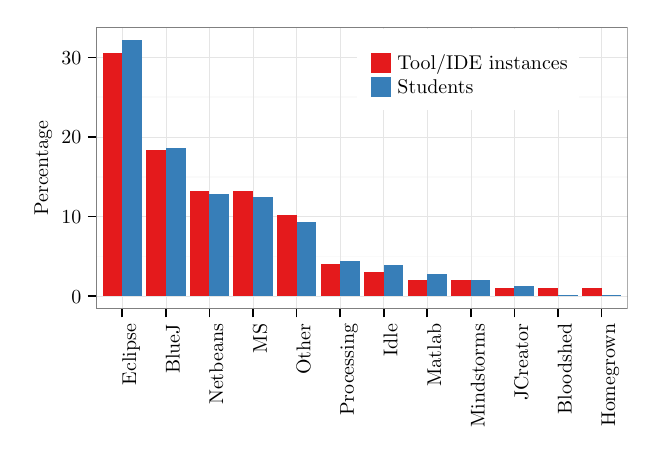
\begin{tikzpicture}[x=1pt,y=1pt]
\definecolor{fillColor}{RGB}{255,255,255}
\path[use as bounding box,fill=fillColor,fill opacity=0.00] (0,0) rectangle (216.81,144.54);
\begin{scope}
\path[clip] (  0.00,  0.00) rectangle (216.81,144.54);
\definecolor{drawColor}{RGB}{255,255,255}
\definecolor{fillColor}{RGB}{255,255,255}

\path[draw=drawColor,line width= 0.6pt,line join=round,line cap=round,fill=fillColor] (  0.00,  0.00) rectangle (216.81,144.54);
\end{scope}
\begin{scope}
\path[clip] ( 24.76, 42.89) rectangle (216.81,144.54);
\definecolor{fillColor}{RGB}{255,255,255}

\path[fill=fillColor] ( 24.76, 42.89) rectangle (216.81,144.54);
\definecolor{drawColor}{gray}{0.98}

\path[draw=drawColor,line width= 0.6pt,line join=round] ( 24.76, 61.89) --
	(216.81, 61.89);

\path[draw=drawColor,line width= 0.6pt,line join=round] ( 24.76, 90.65) --
	(216.81, 90.65);

\path[draw=drawColor,line width= 0.6pt,line join=round] ( 24.76,119.42) --
	(216.81,119.42);
\definecolor{drawColor}{gray}{0.90}

\path[draw=drawColor,line width= 0.2pt,line join=round] ( 24.76, 47.51) --
	(216.81, 47.51);

\path[draw=drawColor,line width= 0.2pt,line join=round] ( 24.76, 76.27) --
	(216.81, 76.27);

\path[draw=drawColor,line width= 0.2pt,line join=round] ( 24.76,105.04) --
	(216.81,105.04);

\path[draw=drawColor,line width= 0.2pt,line join=round] ( 24.76,133.80) --
	(216.81,133.80);

\path[draw=drawColor,line width= 0.2pt,line join=round] ( 34.20, 42.89) --
	( 34.20,144.54);

\path[draw=drawColor,line width= 0.2pt,line join=round] ( 49.94, 42.89) --
	( 49.94,144.54);

\path[draw=drawColor,line width= 0.2pt,line join=round] ( 65.69, 42.89) --
	( 65.69,144.54);

\path[draw=drawColor,line width= 0.2pt,line join=round] ( 81.43, 42.89) --
	( 81.43,144.54);

\path[draw=drawColor,line width= 0.2pt,line join=round] ( 97.17, 42.89) --
	( 97.17,144.54);

\path[draw=drawColor,line width= 0.2pt,line join=round] (112.91, 42.89) --
	(112.91,144.54);

\path[draw=drawColor,line width= 0.2pt,line join=round] (128.65, 42.89) --
	(128.65,144.54);

\path[draw=drawColor,line width= 0.2pt,line join=round] (144.40, 42.89) --
	(144.40,144.54);

\path[draw=drawColor,line width= 0.2pt,line join=round] (160.14, 42.89) --
	(160.14,144.54);

\path[draw=drawColor,line width= 0.2pt,line join=round] (175.88, 42.89) --
	(175.88,144.54);

\path[draw=drawColor,line width= 0.2pt,line join=round] (191.62, 42.89) --
	(191.62,144.54);

\path[draw=drawColor,line width= 0.2pt,line join=round] (207.36, 42.89) --
	(207.36,144.54);
\definecolor{fillColor}{RGB}{228,26,28}

\path[fill=fillColor] ( 27.12, 47.51) rectangle ( 34.20,135.56);
\definecolor{fillColor}{RGB}{55,126,184}

\path[fill=fillColor] ( 34.20, 47.51) rectangle ( 41.29,139.92);
\definecolor{fillColor}{RGB}{228,26,28}

\path[fill=fillColor] ( 42.86, 47.51) rectangle ( 49.94,100.34);
\definecolor{fillColor}{RGB}{55,126,184}

\path[fill=fillColor] ( 49.94, 47.51) rectangle ( 57.03,101.03);
\definecolor{fillColor}{RGB}{228,26,28}

\path[fill=fillColor] ( 58.60, 47.51) rectangle ( 65.69, 85.67);
\definecolor{fillColor}{RGB}{55,126,184}

\path[fill=fillColor] ( 65.69, 47.51) rectangle ( 72.77, 84.36);
\definecolor{fillColor}{RGB}{228,26,28}

\path[fill=fillColor] ( 74.34, 47.51) rectangle ( 81.43, 85.67);
\definecolor{fillColor}{RGB}{55,126,184}

\path[fill=fillColor] ( 81.43, 47.51) rectangle ( 88.51, 83.28);
\definecolor{fillColor}{RGB}{228,26,28}

\path[fill=fillColor] ( 90.09, 47.51) rectangle ( 97.17, 76.86);
\definecolor{fillColor}{RGB}{55,126,184}

\path[fill=fillColor] ( 97.17, 47.51) rectangle (104.25, 74.44);
\definecolor{fillColor}{RGB}{228,26,28}

\path[fill=fillColor] (105.83, 47.51) rectangle (112.91, 59.25);
\definecolor{fillColor}{RGB}{55,126,184}

\path[fill=fillColor] (112.91, 47.51) rectangle (120.00, 60.31);
\definecolor{fillColor}{RGB}{228,26,28}

\path[fill=fillColor] (121.57, 47.51) rectangle (128.65, 56.32);
\definecolor{fillColor}{RGB}{55,126,184}

\path[fill=fillColor] (128.65, 47.51) rectangle (135.74, 58.61);
\definecolor{fillColor}{RGB}{228,26,28}

\path[fill=fillColor] (137.31, 47.51) rectangle (144.40, 53.38);
\definecolor{fillColor}{RGB}{55,126,184}

\path[fill=fillColor] (144.40, 47.51) rectangle (151.48, 55.56);
\definecolor{fillColor}{RGB}{228,26,28}

\path[fill=fillColor] (153.05, 47.51) rectangle (160.14, 53.38);
\definecolor{fillColor}{RGB}{55,126,184}

\path[fill=fillColor] (160.14, 47.51) rectangle (167.22, 53.24);
\definecolor{fillColor}{RGB}{228,26,28}

\path[fill=fillColor] (168.80, 47.51) rectangle (175.88, 50.45);
\definecolor{fillColor}{RGB}{55,126,184}

\path[fill=fillColor] (175.88, 47.51) rectangle (182.96, 51.09);
\definecolor{fillColor}{RGB}{228,26,28}

\path[fill=fillColor] (184.54, 47.51) rectangle (191.62, 50.45);
\definecolor{fillColor}{RGB}{55,126,184}

\path[fill=fillColor] (191.62, 47.51) rectangle (198.71, 47.96);
\definecolor{fillColor}{RGB}{228,26,28}

\path[fill=fillColor] (200.28, 47.51) rectangle (207.36, 50.45);
\definecolor{fillColor}{RGB}{55,126,184}

\path[fill=fillColor] (207.36, 47.51) rectangle (214.45, 47.96);
\definecolor{drawColor}{gray}{0.50}

\path[draw=drawColor,line width= 0.6pt,line join=round,line cap=round] ( 24.76, 42.89) rectangle (216.81,144.54);
\end{scope}
\begin{scope}
\path[clip] (  0.00,  0.00) rectangle (216.81,144.54);
\definecolor{drawColor}{RGB}{0,0,0}

\node[text=drawColor,anchor=base east,inner sep=0pt, outer sep=0pt, scale=  0.72] at ( 19.36, 45.03) {0};

\node[text=drawColor,anchor=base east,inner sep=0pt, outer sep=0pt, scale=  0.72] at ( 19.36, 73.79) {10};

\node[text=drawColor,anchor=base east,inner sep=0pt, outer sep=0pt, scale=  0.72] at ( 19.36,102.56) {20};

\node[text=drawColor,anchor=base east,inner sep=0pt, outer sep=0pt, scale=  0.72] at ( 19.36,131.32) {30};
\end{scope}
\begin{scope}
\path[clip] (  0.00,  0.00) rectangle (216.81,144.54);
\definecolor{drawColor}{RGB}{0,0,0}

\path[draw=drawColor,line width= 0.6pt,line join=round] ( 21.76, 47.51) --
	( 24.76, 47.51);

\path[draw=drawColor,line width= 0.6pt,line join=round] ( 21.76, 76.27) --
	( 24.76, 76.27);

\path[draw=drawColor,line width= 0.6pt,line join=round] ( 21.76,105.04) --
	( 24.76,105.04);

\path[draw=drawColor,line width= 0.6pt,line join=round] ( 21.76,133.80) --
	( 24.76,133.80);
\end{scope}
\begin{scope}
\path[clip] (  0.00,  0.00) rectangle (216.81,144.54);
\definecolor{drawColor}{RGB}{0,0,0}

\path[draw=drawColor,line width= 0.6pt,line join=round] ( 34.20, 39.89) --
	( 34.20, 42.89);

\path[draw=drawColor,line width= 0.6pt,line join=round] ( 49.94, 39.89) --
	( 49.94, 42.89);

\path[draw=drawColor,line width= 0.6pt,line join=round] ( 65.69, 39.89) --
	( 65.69, 42.89);

\path[draw=drawColor,line width= 0.6pt,line join=round] ( 81.43, 39.89) --
	( 81.43, 42.89);

\path[draw=drawColor,line width= 0.6pt,line join=round] ( 97.17, 39.89) --
	( 97.17, 42.89);

\path[draw=drawColor,line width= 0.6pt,line join=round] (112.91, 39.89) --
	(112.91, 42.89);

\path[draw=drawColor,line width= 0.6pt,line join=round] (128.65, 39.89) --
	(128.65, 42.89);

\path[draw=drawColor,line width= 0.6pt,line join=round] (144.40, 39.89) --
	(144.40, 42.89);

\path[draw=drawColor,line width= 0.6pt,line join=round] (160.14, 39.89) --
	(160.14, 42.89);

\path[draw=drawColor,line width= 0.6pt,line join=round] (175.88, 39.89) --
	(175.88, 42.89);

\path[draw=drawColor,line width= 0.6pt,line join=round] (191.62, 39.89) --
	(191.62, 42.89);

\path[draw=drawColor,line width= 0.6pt,line join=round] (207.36, 39.89) --
	(207.36, 42.89);
\end{scope}
\begin{scope}
\path[clip] (  0.00,  0.00) rectangle (216.81,144.54);
\definecolor{drawColor}{RGB}{0,0,0}

\node[text=drawColor,rotate= 90.00,anchor=base east,inner sep=0pt, outer sep=0pt, scale=  0.72] at ( 39.16, 37.49) {Eclipse};

\node[text=drawColor,rotate= 90.00,anchor=base east,inner sep=0pt, outer sep=0pt, scale=  0.72] at ( 54.90, 37.49) {BlueJ};

\node[text=drawColor,rotate= 90.00,anchor=base east,inner sep=0pt, outer sep=0pt, scale=  0.72] at ( 70.65, 37.49) {Netbeans};

\node[text=drawColor,rotate= 90.00,anchor=base east,inner sep=0pt, outer sep=0pt, scale=  0.72] at ( 86.39, 37.49) {MS};

\node[text=drawColor,rotate= 90.00,anchor=base east,inner sep=0pt, outer sep=0pt, scale=  0.72] at (102.13, 37.49) {Other};

\node[text=drawColor,rotate= 90.00,anchor=base east,inner sep=0pt, outer sep=0pt, scale=  0.72] at (117.87, 37.49) {Processing};

\node[text=drawColor,rotate= 90.00,anchor=base east,inner sep=0pt, outer sep=0pt, scale=  0.72] at (133.61, 37.49) {Idle};

\node[text=drawColor,rotate= 90.00,anchor=base east,inner sep=0pt, outer sep=0pt, scale=  0.72] at (149.36, 37.49) {Matlab};

\node[text=drawColor,rotate= 90.00,anchor=base east,inner sep=0pt, outer sep=0pt, scale=  0.72] at (165.10, 37.49) {Mindstorms};

\node[text=drawColor,rotate= 90.00,anchor=base east,inner sep=0pt, outer sep=0pt, scale=  0.72] at (180.84, 37.49) {JCreator};

\node[text=drawColor,rotate= 90.00,anchor=base east,inner sep=0pt, outer sep=0pt, scale=  0.72] at (196.58, 37.49) {Bloodshed};

\node[text=drawColor,rotate= 90.00,anchor=base east,inner sep=0pt, outer sep=0pt, scale=  0.72] at (212.32, 37.49) {Homegrown};
\end{scope}
\begin{scope}
\path[clip] (  0.00,  0.00) rectangle (216.81,144.54);
\definecolor{drawColor}{RGB}{0,0,0}

\node[text=drawColor,rotate= 90.00,anchor=base,inner sep=0pt, outer sep=0pt, scale=  0.72] at (  7.36, 93.72) {Percentage};
\end{scope}
\begin{scope}
\path[clip] (  0.00,  0.00) rectangle (216.81,144.54);
\definecolor{fillColor}{RGB}{255,255,255}

\path[fill=fillColor] (119.02,114.68) rectangle (199.37,143.90);
\end{scope}
\begin{scope}
\path[clip] (  0.00,  0.00) rectangle (216.81,144.54);
\definecolor{fillColor}{RGB}{228,26,28}

\path[fill=fillColor] (124.00,128.20) rectangle (131.11,135.31);
\end{scope}
\begin{scope}
\path[clip] (  0.00,  0.00) rectangle (216.81,144.54);
\definecolor{fillColor}{RGB}{55,126,184}

\path[fill=fillColor] (124.00,119.66) rectangle (131.11,126.77);
\end{scope}
\begin{scope}
\path[clip] (  0.00,  0.00) rectangle (216.81,144.54);
\definecolor{drawColor}{RGB}{0,0,0}

\node[text=drawColor,anchor=base west,inner sep=0pt, outer sep=0pt, scale=  0.72] at (133.63,129.27) {Tool/IDE instances};
\end{scope}
\begin{scope}
\path[clip] (  0.00,  0.00) rectangle (216.81,144.54);
\definecolor{drawColor}{RGB}{0,0,0}

\node[text=drawColor,anchor=base west,inner sep=0pt, outer sep=0pt, scale=  0.72] at (133.63,120.74) {Students};
\end{scope}
\end{tikzpicture}
